\documentclass{article}

\usepackage[T1]{fontenc}
\usepackage[utf8]{inputenc}
\usepackage{lmodern,textcomp}
\usepackage[francais]{babel}
\usepackage{amsmath}
\usepackage{graphicx}
\usepackage{listings} % code source
\usepackage{color}
 
\definecolor{codegreen}{rgb}{0,0.6,0}
\definecolor{codegray}{rgb}{0.5,0.5,0.5}
\definecolor{codepurple}{rgb}{0.58,0,0.82}
\definecolor{backcolor}{rgb}{0.95,0.95,0.92}
 
% Couleur pour le code source
\lstdefinestyle{mystyle}{
    backgroundcolor=\color{backcolor},   
    commentstyle=\color{codegreen},
    keywordstyle=\color{magenta},
    numberstyle=\tiny\color{codegray},
    stringstyle=\color{codepurple},
    basicstyle=\footnotesize,
    breakatwhitespace=false,         
    breaklines=true,                 
    captionpos=b,                    
    keepspaces=true,                 
    numbers=left,                    
    numbersep=5pt,                  
    showspaces=false,                
    showstringspaces=false,
    showtabs=false,                  
    tabsize=2,
}

\lstset{
	frame=simple,
	texcl=true,
	extendedchars=true,
	style=mystyle,
	language=C++,
}

% Inutile ?
\lstset{literate=
  {á}{{\'a}}1 {é}{{\'e}}1 {í}{{\'i}}1 {ó}{{\'o}}1 {ú}{{\'u}}1
  {Á}{{\'A}}1 {É}{{\'E}}1 {Í}{{\'I}}1 {Ó}{{\'O}}1 {Ú}{{\'U}}1
  {à}{{\`a}}1 {è}{{\`e}}1 {ì}{{\`i}}1 {ò}{{\`o}}1 {ù}{{\`u}}1
  {À}{{\`A}}1 {È}{{\'E}}1 {Ì}{{\`I}}1 {Ò}{{\`O}}1 {Ù}{{\`U}}1
  {ä}{{\"a}}1 {ë}{{\"e}}1 {ï}{{\"i}}1 {ö}{{\"o}}1 {ü}{{\"u}}1
  {Ä}{{\"A}}1 {Ë}{{\"E}}1 {Ï}{{\"I}}1 {Ö}{{\"O}}1 {Ü}{{\"U}}1
  {â}{{\^a}}1 {ê}{{\^e}}1 {î}{{\^i}}1 {ô}{{\^o}}1 {û}{{\^u}}1
  {Â}{{\^A}}1 {Ê}{{\^E}}1 {Î}{{\^I}}1 {Ô}{{\^O}}1 {Û}{{\^U}}1
  {œ}{{\oe}}1 {Œ}{{\OE}}1 {æ}{{\ae}}1 {Æ}{{\AE}}1 {ß}{{\ss}}1
  {ű}{{\H{u}}}1 {Ű}{{\H{U}}}1 {ő}{{\H{o}}}1 {Ő}{{\H{O}}}1
  {ç}{{\c c}}1 {Ç}{{\c C}}1 {ø}{{\o}}1 {å}{{\r a}}1 {Å}{{\r A}}1
  {€}{{\euro}}1 {£}{{\pounds}}1 {«}{{\guillemotleft}}1
  {»}{{\guillemotright}}1 {ñ}{{\~n}}1 {Ñ}{{\~N}}1 {¿}{{?`}}1
}

\begin{document}

\subsection{Détection d'ensembles d'une même couleur} % TODO: Trouver un nouveau sous-titre
Une autre approche pour détecter des pièces de monnaie sur une image est d'exploiter le contraste entre les pièces elles-mêmes et le matériau sur lequel elles sont placées. Dans l'image suivante, par exemple, les pièces sont jaune ou rouge foncé alors que le fond est blanc.

\begin{center}
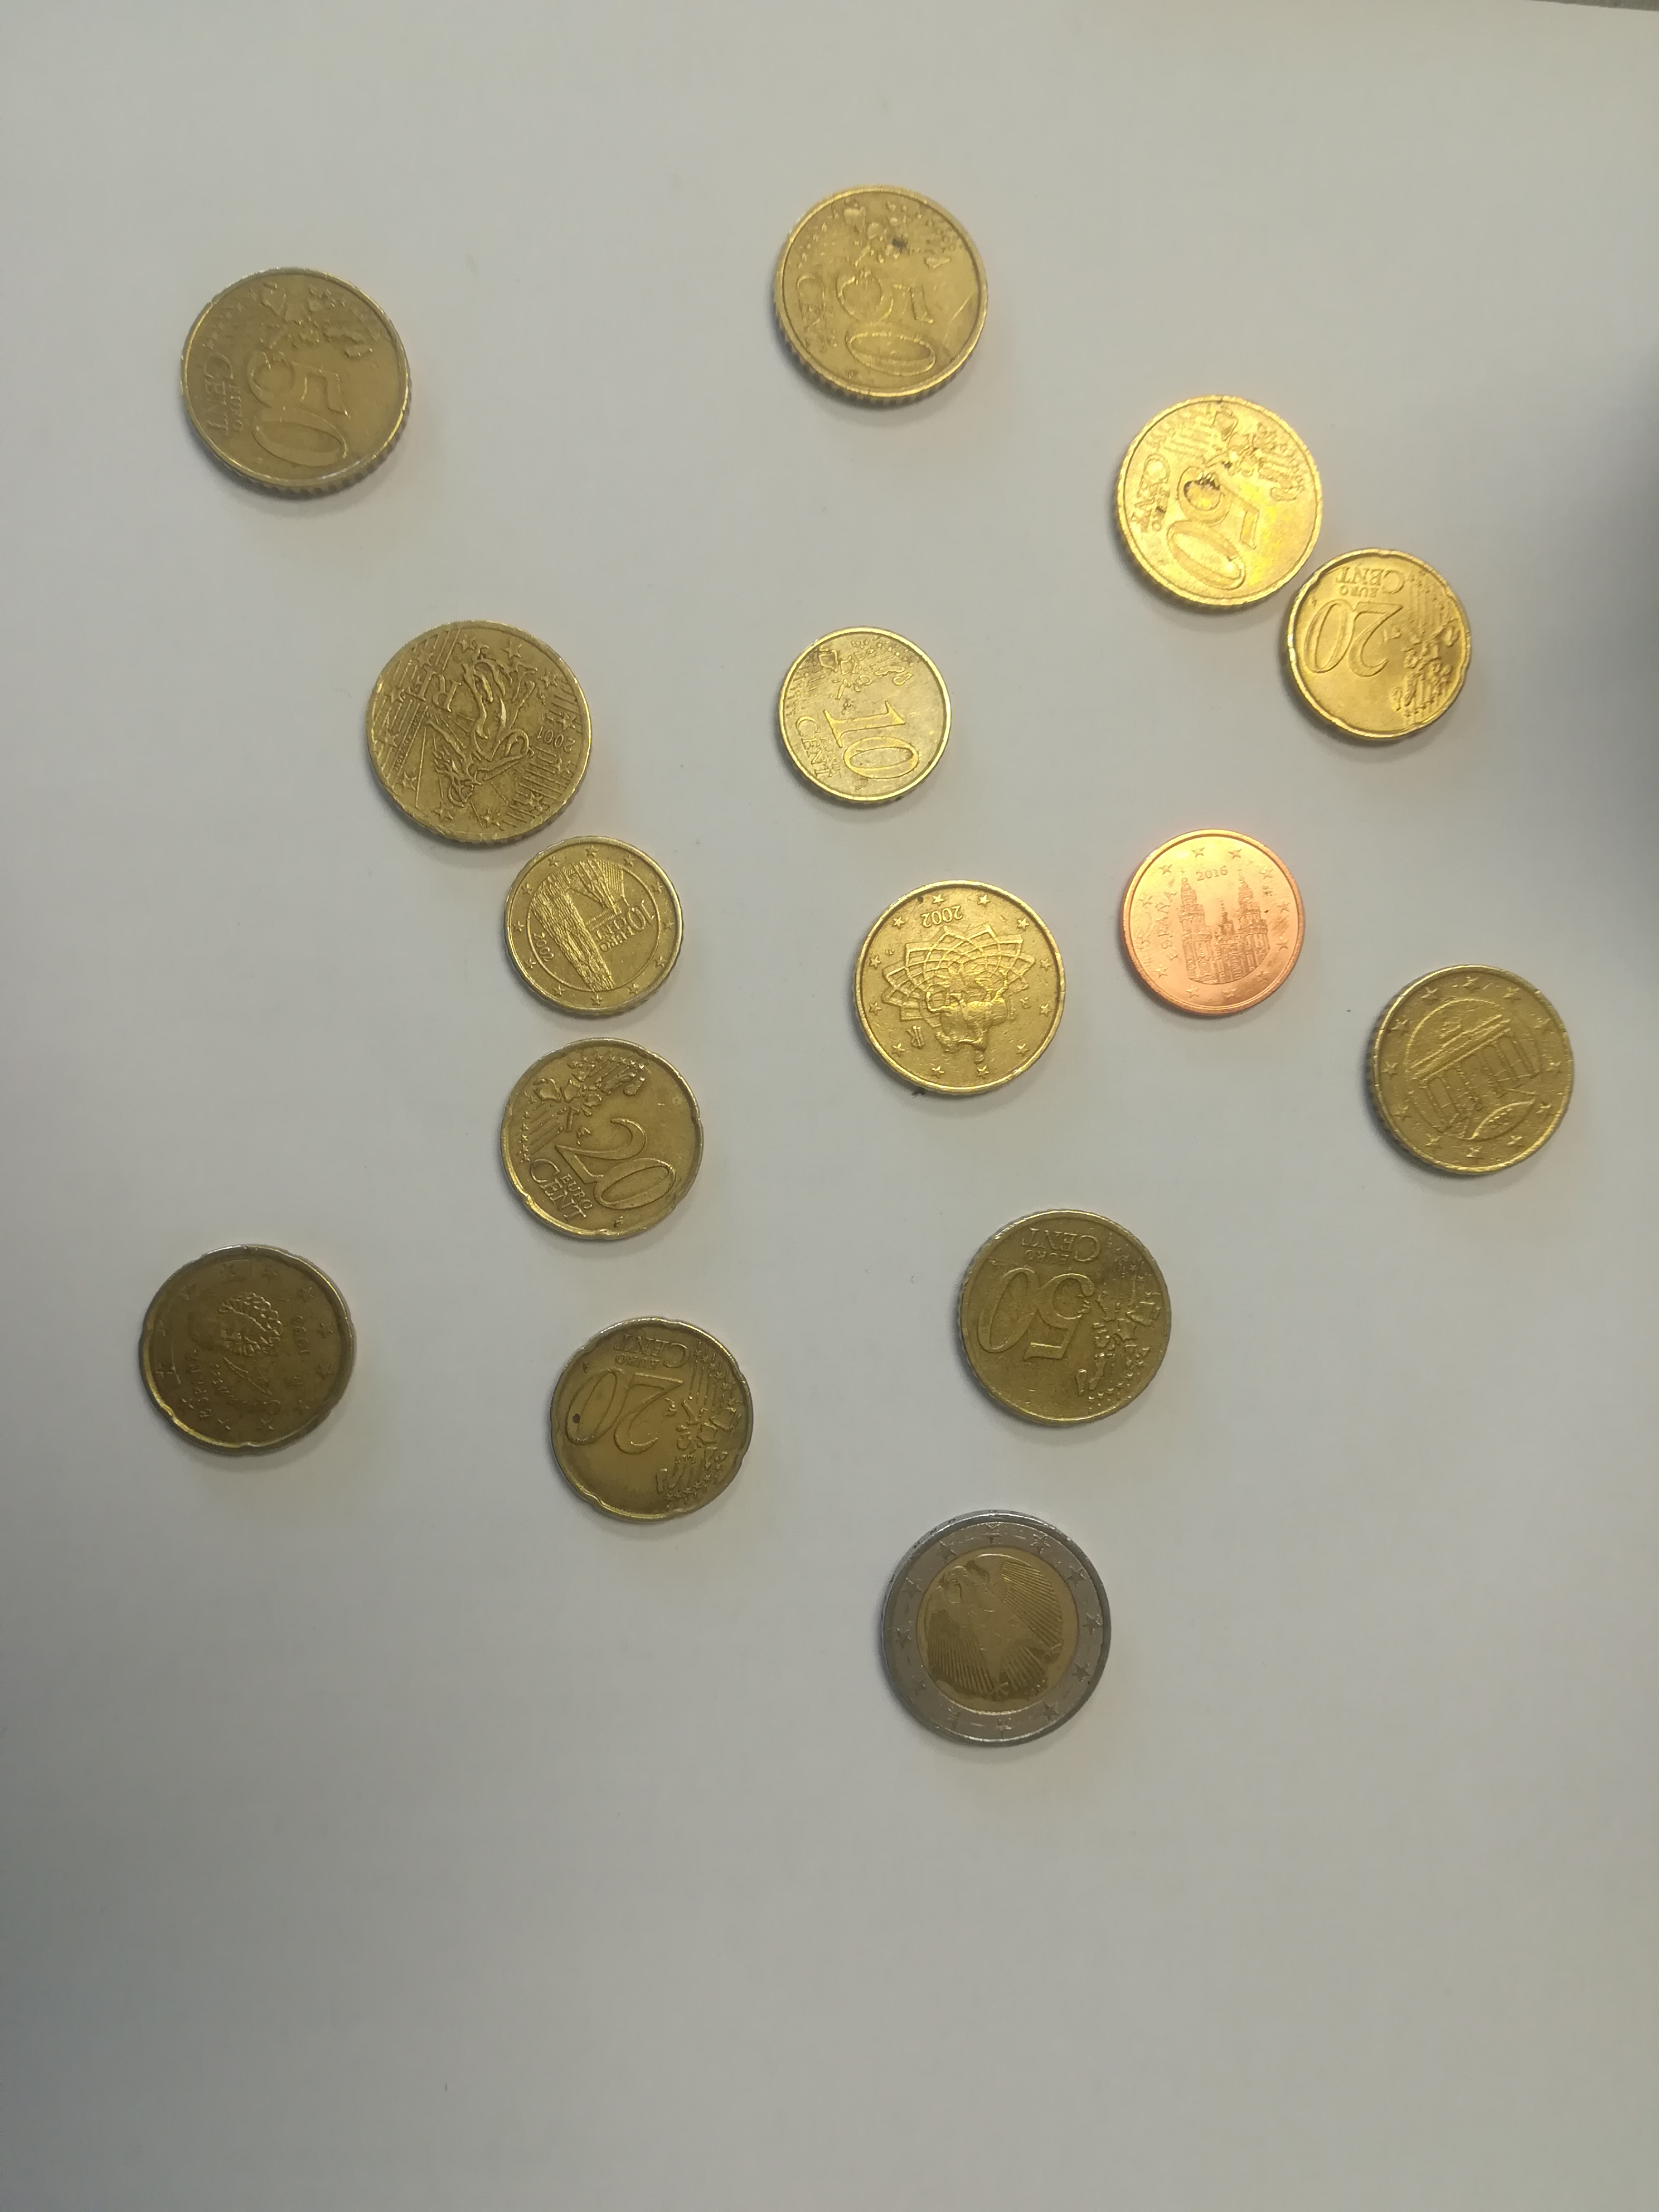
\includegraphics[width=0.5\linewidth]{images/manycoins.png}
\end{center}

Nous allons développer un algorithme permettant d'utiliser la couleur du fond pour isoler les pièces. Et nous allons l'appliquer à cette image afin d'en extraire les pièces.

\section{Un algorithme en profondeur}
\subsection{Généralités sur les graphes}

Un graphe est un ensemble de points appelés \textit{sommets} (\textit{\textbf{v}ertices} en anglais) et de connections appelées \textit{arêtes} (\textit{\textbf{e}dges} en anglais). Voici par exemple un graphe de $6$ sommets et de $7$ arêtes:

\begin{center}
\includegraphics[width=0.5\linewidth]{images/graph.png}
\end{center}

Dans ce cas-ci, les points sont $1, 2, 3, 4, 5, 6$ et les connections sont \\ $(1,2),(1,5),(2,3),(2,5),(3,4),(4,5),(4,6)$. \\
D'un point de vue mathématique, le \textbf{g}raphe G peut se définir ainsi: 
$$\begin{array}{l}
G = (V, E), \\
V = \{1,2,3,4,5,6\}, \\
E = \{(1,2),(1,5),(2,3),(2,5),(3,4),(4,5),(4,6)\}.
\end{array}$$

% TODO: définir chemin, sommet adjacent

\subsection{Composantes connexes}
Le graphe ci-dessus est un exemple de graphe \textit{connexe}, c'est-à-dire un graph dont tout point est relié à tout point. Il existe aussi des graphes non connexes. Les différentes parties connexes du graphe sont alors appelées des \textit{composantes connexes}. Le graphe ci-dessous est ainsi composé de $3$ composantes connexes. Il est clair que le graphe est non connexe car le point $1$ n'est par exemple pas relié au point $3$.

\begin{center}
\includegraphics[width=0.5\linewidth]{images/3-components.png}
\end{center}

\subsection{Parcours d'un graphe}
\paragraph{}
Voyons maintenant comment on peut détecter les différentes composantes connexes d'un graphe. Pour ce faire, commençons par remarquer la transitivité de la définition d'une composante connexe. En effet, s'il existe un chemin de $u$ à $v$ et de $u$ à $w$, il existe forcément un chemin allant de $v$ à $w$ et inversément. Il suffit en effet de partir de $v$, de se rendre à $u$ et de rejoindre $w$ depuis $u$. Cette propriété peut sembler anodine, mais elle affirme que pour détecter une composante connexe, il suffit de partir d'un sommet quelconque et de parcourir le graphe en catalogant tous les sommets atteignables.

\paragraph{}
Un algorithme classique pour parcourir les graphes est le \textit{depth-first search} (DFS) ou encore \textit{parcours en profondeur}, appelé ainsi parce qu'il va aussi loin qu'il peut avant de revenir en arrière. \\
On part d'un sommet $u$. Si le sommet $u$ n'a pas encore été visité, on le marque comme visité. Ensuite, pour chaque sommet $v$ adjacent à $u$, on reprend l'algorithme récursivement. En C++, cela donne:

\lstinputlisting[caption=DFS]{src/simple-dfs.cpp}

\paragraph{}
Cet algorithme ne parcourt qu'une seule composante connexe. Afin de détecter toutes les composantes connexes, on peut essayer de lancer l'algorithme depuis chaque sommet. Si l'algorithme n'a pas encore été lancé depuis un sommet $u$, c'est que $u$ appartient à une nouvelle composante connexe.

\lstinputlisting[caption=Composantes connexes]{src/simple-dfs-call.cpp}

\paragraph{}
Ce code parcourt bien tous les sommets mais il ne permet toujours pas de déterminer la composante connexe d'un sommet donné. Réglons ce problème: plutôt que d'enregistrer si un sommet a été visité ou non, on peut directement enregistrer à quelle composante connexe il appartient.

\lstinputlisting[caption=Composantes connexes]{src/simple-cc-full.cpp}

\end{document}
